% Chapter: HyperAgents
% Adapted from: Zhang, Zhao, Yang, Foerster, Clune, Jiang, Devlin, Shavrina.
% "HyperAgents." arXiv / NeurIPS 2026.
% Co-first authors: Jenny Zhang, Bingchen Zhao, Wannan Yang.
%
% This chapter is a reprint of: \\
% Zhang$^*$, Zhao$^*$, Yang$^*$, Foerster, Clune, Jiang, Devlin, Shavrina.
% \textit{NeurIPS 2026}.

This chapter is a reprint of: \\
Zhang$^{*}$, Zhao$^{*}$, Yang$^{*}$, Foerster, Clune, Jiang, Devlin, Shavrina.
\textit{NeurIPS 2026}. ($^{*}$equal contribution)

\section*{Abstract}

Self-improving AI systems aim to reduce reliance on human engineering by learning to improve their own learning and problem-solving processes. Existing approaches to self-improvement rely on fixed, handcrafted meta-level mechanisms, fundamentally limiting how fast such systems can improve. The Darwin G\"{o}del Machine (DGM) achieves open-ended self-improvement in coding, but this relies on domain-specific alignment between task performance and self-modification skill. However, this alignment does not generally hold beyond coding domains. We introduce \textbf{hyperagents}, self-referential agents that integrate a task agent (which solves the target task) and a meta agent (which modifies itself and the task agent) into a single editable program. Crucially, the meta-level modification procedure is itself editable, enabling metacognitive self-modification, improving not only the task-solving behavior, but also the mechanism that generates future improvements. We instantiate this framework by extending DGM to create DGM-Hyperagents (DGM-H), eliminating the need for domain-specific alignment to potentially support self-accelerating progress on any computable task. Across diverse domains, the DGM-H improves performance over time and outperforms baselines without self-improvement or open-ended exploration, as well as prior self-improving systems. Furthermore, the DGM-H improves the process by which it generates new agents (e.g., persistent memory, performance tracking), and these meta-level improvements transfer across domains and accumulate across runs. All experiments were conducted with safety precautions (e.g., sandboxing, human oversight). We discuss what safety entails in this setting and the broader implications of self-improving systems. DGM-Hyperagents offer a glimpse of open-ended AI systems that do not merely search for better solutions, but continually improve their search for how to improve.

\section{Introduction}
\label{sec:intro}

With appropriate safety considerations, AI systems that can improve themselves could transform scientific progress from a human-paced process into an autonomously accelerating one, thereby allowing society to realize the benefits of technological advances much earlier. Such self-improving AI seeks to continually improve its own learning and task-solving abilities. However, most existing self-improvement architectures rely on a fixed meta agent (i.e., a higher-level system that modifies a base system). This creates a limitation since the base system can only be improved within the boundaries defined by the meta agent's design. Adding a meta-meta system to improve the meta agent does not solve this problem, it merely shifts the issue upward and ultimately leads to an infinite regress of meta-levels. To overcome this limitation and allow a system to modify any part of itself without being constrained by its initial implementation, the system must be self-referential, that is, able to analyze, modify, and evaluate itself \citep{kirsch2022eliminating, zhang2025darwin}. When the mechanism of improvement is itself subject to improvement, progress can become self-accelerating and potentially unbounded \citep{lu2023arbitrary}.

The Darwin G\"{o}del Machine (DGM) \citep{zhang2025darwin} demonstrates that open-ended self-improvement is achievable in coding, where agents generate and evaluate modifications to their own code, retaining successful variants in an archive as stepping stones. However, the DGM relies on a fixed, handcrafted instruction-generation mechanism that is not itself modifiable, bottlenecking its capacity for self-improvement (Appendix~\ref{app:baseline-details}). Moreover, the DGM's ability to improve at self-improving depends on an alignment assumption: that the skills required to solve evaluation tasks are the same as those needed for effective self-modification. This assumption is unlikely to hold outside coding domains (Section~\ref{sec:related-work}).

This work introduces \textit{hyperagents}, self-referential agents that can in principle self-improve for any computable task. Here, an \textit{agent} is any computable program, optionally including calls to foundation models (FMs), external tools, or learned components. A \textit{task agent} solves a given task. A \textit{meta agent} modifies agents and generates new ones. A hyperagent combines the task agent and the meta agent into a single self-referential, modifiable program, such that the mechanism responsible for generating improvements is itself subject to modification. As a result, a hyperagent can improve not only how it solves tasks (i.e., the task agent), but also how it generates and applies future modifications (i.e., the meta agent). Because its self-improvement mechanism is itself modifiable, we call this \textit{metacognitive self-modification}.

We extend the DGM with hyperagents, creating DGM-Hyperagents (DGM-H). The DGM-H retains the open-ended exploration structure of the DGM and extends the DGM with metacognitive self-modification. As with DGM, to support sustained progress and avoid premature convergence, the DGM-H grows an archive of hyperagents by branching from selected candidates, allowing them to self-modify, evaluating the resulting hyperagents, and adding them back to the archive. Because a hyperagent can modify its self-modification process, the DGM-H is not constrained by its initial implementation and can potentially self-improve for any computable task.

Across our experiments, the DGM-H demonstrates substantial and generalizable improvements in both task performance and self-improvement ability. On the Polyglot coding benchmark \citep{gauthier2024polyglot}, the DGM-H achieves gains comparable to the most established prior self-improving algorithm \citep[the Darwin G\"{o}del Machine,][]{zhang2025darwin}, despite not being handcrafted for coding. Beyond coding, the DGM-H substantially improves performance on paper review \citep{zhao2026apres} and robotics reward design \citep{genesis2024}, with gains transferring to held-out test tasks and significantly outperforming prior self-improving algorithms, which struggle outside coding unless customized. Ablations without self-improvement or without open-ended exploration show little to no progress, highlighting the necessity of each component (Section~\ref{sec:results-task}). Crucially, the DGM-H learns transferable mechanisms on how to self-improve (e.g., persistent memory, performance tracking) that systematically improve its ability to generate better task or meta agents over time. As a result, meta-level improvements learned by the DGM-H transfer across domains. Specifically, hyperagents optimized in one setting (i.e., paper review and robotics tasks) remain significantly effective at generating improved task agents in a different domain (i.e., Olympiad-level math grading) (Section~\ref{sec:results-meta}). We further show that self-improvements learned by the DGM-H in one setting can compound with continued self-improvement in another setting (Section~\ref{sec:results-compound}). This suggests that, given appropriate tasks, the DGM-H has the potential to achieve unbounded open-ended self-improvement over time.

We discuss the safety implications of such open-ended self-improving systems and outline practical considerations for responsible deployment in Appendix~\ref{app:safety}. Overall, hyperagents open up the possibility of improving their ability to improve while improving their ability to perform any computable task.

\section{Related Work}
\label{sec:related-work}

\textbf{Self-improving AI.}
Early theoretical work on self-improving AI dates back to formal models of self-modifying agents \citep{hutter2003gentle}. One prominent example is the G\"{o}del Machine \citep{schmidhuber2003godel}, which proposes agents that rewrite themselves when provably beneficial, though such approaches remain impractical in real-world settings. Subsequent research explored self-improvement through adaptive neural systems, in which agents modify their own weights or learning dynamics via meta-learning \citep{schmidhuber1993neural, miconi2018differentiable, javed2019meta, beaulieu2020learning, miconi2020backpropamine, irie2022modern, chalvidal2022meta, oh2025discovering}, evolution \citep{stanley2002evolving, lange2023discovering, qiu2025evolution, zhao2025automated}, or self-play \citep{silver2016mastering, silver2017mastering, xia2025agent0, xia2026skillrl}. Notably, \citet{silver2017mastering} use self-play to iteratively improve neural network agents, achieving superhuman performance in domains such as Go and chess, although the underlying learning algorithms themselves remain fixed and human-designed. More recently, FMs have enabled self-improvement through iterative refinement of prompts \citep{fernando2023promptbreeder, wang2025evolving, zhang2025agentic, zhang2025recursive, ye2026meta}, reasoning traces \citep{zelikman2022star, yin2025godel, havrilla2024teaching, zhuge2024gptswarm}, and entire code repositories \citep{zhang2025darwin, wang2025huxley, xia2025live}, as well as through systems that update model weights using self-generated data or interaction \citep{wu2024copilot, zweiger2025self, wen2025unsupervised, wei2025toward}. Among these, the Darwin G\"{o}del Machine (DGM) \citep{zhang2025darwin} stands out as a practical instantiation of recursive self-improvement in coding domains. However, despite their effectiveness, most existing approaches (including the DGM and its derivatives) rely on fixed, handcrafted meta-level mechanisms (Appendix~\ref{app:baseline-details}) that constrain how self-improvement can compound over time and generalize across domains.

\textbf{Self-referential meta-learning.}
Self-referential meta-learning studies systems that learn to improve the mechanisms by which learning occurs. Prior work has explored this idea in neural networks \citep{kirsch2022eliminating, jackson2024discovering} and evolutionary methods \citep{lu2023arbitrary}. More recently, several works have explored self-referential improvement using FM-based agents \citep{zelikman2024self, robeyns2025self, yin2025godel, zhang2025darwin}. The Darwin G\"{o}del Machine (DGM) \citep{zhang2025darwin} and its successors \citep{wang2025huxley, xia2025live, weng2026group} instantiate recursive self-improvement through self-modification, primarily in coding domains. However, these approaches improve at improving primarily within coding tasks only.

In the DGM and related systems, a coding agent is tasked with improving itself, and the resulting improved coding agent is then used in subsequent self-improvement steps to generate an even better version of itself. Because both the evaluation task and the self-modification process involve coding, improving the coding agent also enhances the system's ability to carry out future self-improvements. However, this property only holds when the evaluation task and the self-modification task are closely aligned. For example, if the evaluation task were instead poetry writing, improving an agent's poetry-writing ability would not necessarily improve its ability to modify its own code. Prior work therefore relies on an \emph{alignment} between the evaluation task and the skills required for self-improvement. In contrast, hyperagents do not assume such alignment, because the self-modification mechanism is fully modifiable and not tied to any particular task domain. Hence, hyperagents can improve both task performance and the process of improvement itself across any computable task.

\section{Methods}
\label{sec:method}

\begin{figure}[ht]
\centering
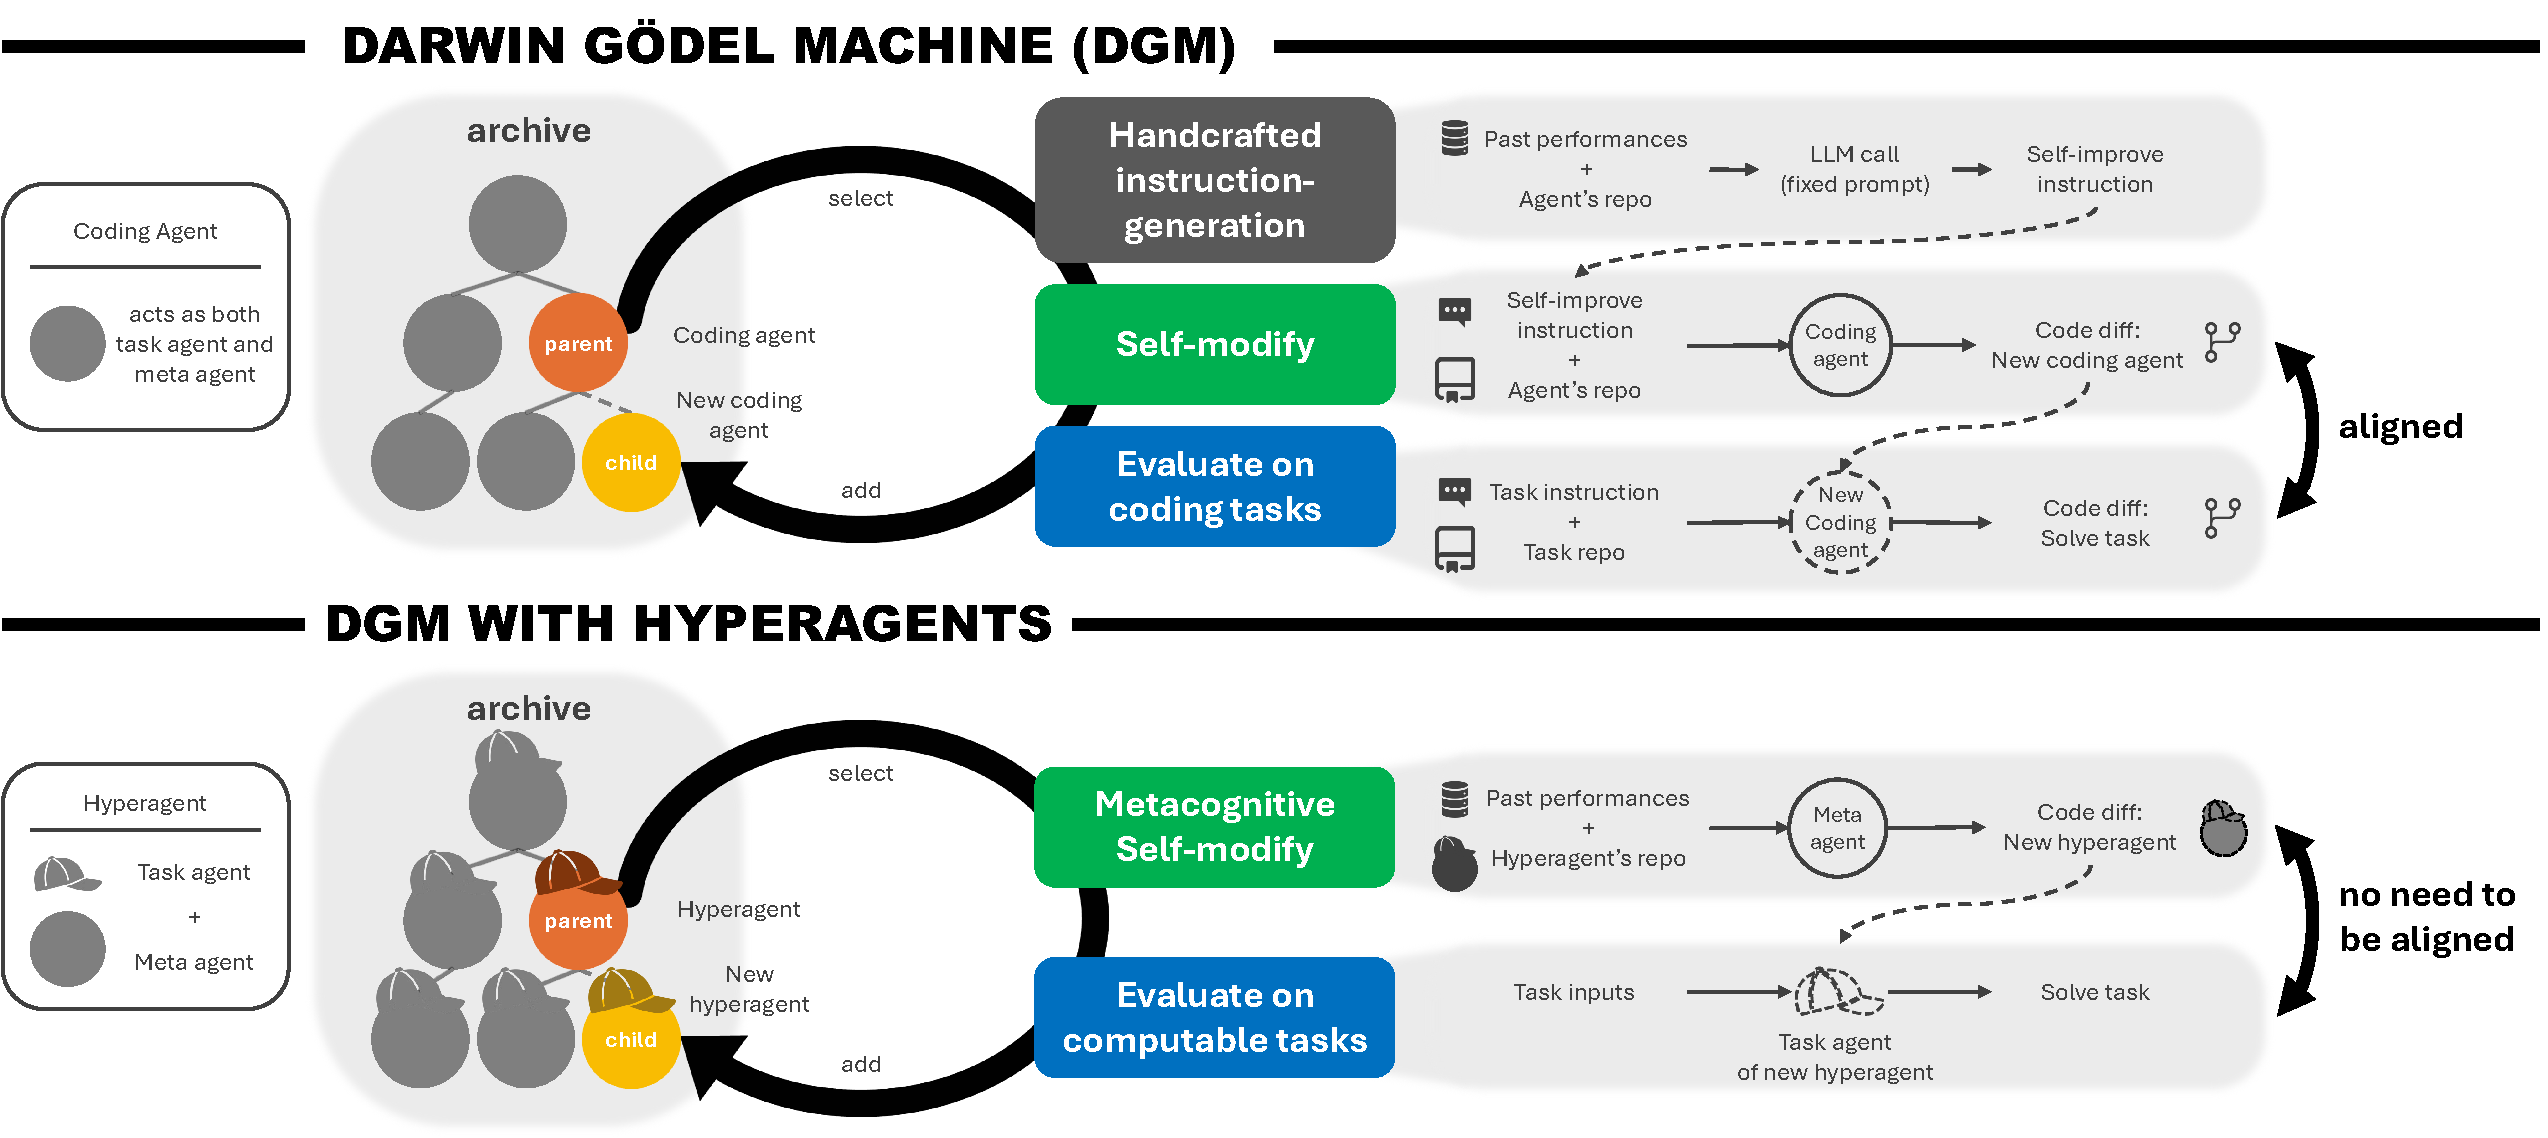
\includegraphics[width=\textwidth]{figures/ch_hyperagents/conceptual.pdf}
\caption[The Darwin G\"{o}del Machine with Hyperagents]{\textbf{The Darwin G\"{o}del Machine with Hyperagents.} The DGM-Hyperagents (DGM-H) extends the Darwin G\"{o}del Machine (DGM) \citep{zhang2025darwin} beyond coding tasks, enabling agents to improve not only their task performance but also their ability to improve themselves, across any computable task. (Top) In the DGM, a coding agent evolves through open-ended exploration by generating and evaluating self-modified variants, which are stored in an archive of stepping stones. The same coding agent acts as both the task agent (to be evaluated) and the meta agent (to generate modifications). While this design enables compounding gains in coding, the instruction-generation mechanism that drives self-improvement is fixed and handcrafted. Consequently, recursive improvement depends on alignment between coding performance and self-modification ability. (Bottom) In the DGM-H, the task agent and meta agent are combined into a single modifiable program called a hyperagent. This design allows the meta agent itself to be autonomously improved. The system retains the open-ended exploration structure of the DGM while making the meta-level improvement mechanism editable. This enables metacognitive self-modification and supports self-referential improvement across any computable task.}
\label{fig:conceptual}
\end{figure}

We introduce hyperagents, self-referential agents that unify task execution and agent generation into a single modifiable program. A hyperagent can improve not only how it solves tasks but also how it generates future improvements. To enable sustained and accumulating progress, we instantiate hyperagents by building directly on the Darwin G\"{o}del Machine (DGM) to form DGM-Hyperagents (DGM-H). The DGM provides an open-ended, population-based exploration process that maintains an archive of progressively improving agents, allowing successful variants to serve as stepping stones for future gains. DGM-H retains this open-ended evolutionary structure and extends it by making the entire meta-level modification mechanism editable (Figure~\ref{fig:conceptual}). By allowing agents to modify not only how they solve tasks but also how they improve themselves, the DGM-H has the potential to open-endedly self-improve on any computable task.

\textbf{Agents.} This paper defines an \textit{agent} as any computable program, optionally including calls to FMs, external tools, or learned components. Agents are not restricted to a particular representation (e.g., neural networks or prompts) and may include arbitrary algorithmic logic, memory, and control flow.
A \textit{task agent} is an agent instantiated to solve a set of tasks. Examples include generating code edits for a software repository \citep{gauthier2024polyglot, jimenez2024swebench}, predicting acceptance decisions for research papers \citep{couto2024relevai}, and designing reward functions for robotics environments \citep{maeureka}. Task agents are evaluated empirically on the given task.
A \textit{meta agent} is an agent whose only task is to modify existing agents and generate new ones. Given access to the entire archive of previous agents and evaluations, a meta agent proposes changes intended to improve future performance (including potentially many generations later). Importantly, these changes may target not only task-solving logic but also the meta agent itself, enabling improvements to the procedures by which future modifications are generated.

\textbf{Hyperagents.} A hyperagent is a self-referential agent that integrates a task agent and a meta agent within a single editable program, enabling it to modify not only how it performs tasks but also how it generates future self-modifications. Unlike hierarchical systems with fixed meta-levels, in hyperagents the meta agent is part of the same editable program and can rewrite itself. As a result, a hyperagent can improve both (1) how it solves tasks and (2) how it generates future self-improvements. We use Python, which is Turing-complete \citep{turing1936computable}, and since a hyperagent can edit any code, it has the potential to build any computable machine.

\textbf{Metacognitive self-modification.} In hyperagents, the agent's self-improvement mechanism is itself subject to modification. In addition to improving its performance on a given task, the agent can simultaneously modify the procedures by which it proposes and applies further self-improvements. We refer to this process as \textit{metacognitive self-modification}, in which the hyperagent improves not only the task-performing agent responsible for solving the given task, but also the meta agent that determines how subsequent hyperagents are generated. This characteristic addresses a central limitation of prior self-improving systems \citep{zhang2025darwin, wang2025huxley} by directly enabling improvements to the self-improvement process itself (Section~\ref{sec:related-work}). Examples of such metacognitive self-modifications are presented in Appendix~\ref{app:qual-meta}.

\textbf{Darwin G\"{o}del Machine with Hyperagents.}
Augmenting the original DGM \citep{zhang2025darwin} with hyperagents, we create DGM-Hyperagents (DGM-H). DGM-H employs the open-ended exploration process in the DGM to mitigate premature convergence and avoid getting trapped in local optima. This process maintains an archive of generated hyperagents, initialized with a single hyperagent and expanded over time by continuously accumulating generated variants. The process alternates between two phases: metacognitive self-modification and evaluation. During the metacognitive self-modification phase, selected parent hyperagents from the archive generate modified versions of themselves. Parent selection is probabilistic and proportional to a hyperagent's performance, and inversely proportional to the number of children that successfully compiled, biasing sampling toward hyperagents that perform well and generate strong descendants while preserving exploration (Appendix~\ref{app:parent-selection}). During the evaluation phase, each modified hyperagent is empirically evaluated and subsequently added to the archive. In principle, a fully self-referential algorithm should allow modification of every part of itself (including the parent selection and evaluation mechanisms). While we present preliminary results exploring the possibility of automatically improving the parent selection mechanism in Appendix~\ref{app:res-parentselect}, the experiments in the main text use a handcrafted parent selection mechanism that is not subject to modification in order to isolate the effects of hyperagent self-modification. Overall, DGM-H consists of two interacting components: (1) an open-ended exploration process inherited from the DGM, and (2) an initial hyperagent, which evolves over time through self-generated variants (Figure~\ref{fig:conceptual}, Appendix~\ref{app:algo-details}). By extending the DGM to make the meta-level mechanism itself modifiable, the DGM-H generalizes recursive self-improvement beyond coding and enables self-referential improvement for any computable task.

\section{Experiment Setup}
\label{sec:exp-setup}

The DGM-H is initialized with a single hyperagent built around a frozen FM \citep{brown2020language} with external tool-use capabilities \citep{schick2023toolformer}. The FM autonomously invokes tools as needed at each step. This initial hyperagent is equipped with two tools: a bash tool for executing shell commands, and a specialized tool for inspecting and modifying files. In the initial hyperagent, the task agent receives the task inputs and outputs the response from a single FM call. The meta agent receives the location of the agent's repository, the location of previous evaluation results, and the number of remaining experiment iterations (the experiment budget is a hyperparameter), and is tasked with modifying any part of the given codebase (Appendix~\ref{app:initial-agent}). We deliberately keep the implementation of the initial hyperagent (i.e., both the task agent and the meta agent) simple, allowing for a broad search space and avoiding prematurely constraining the range of possible improvements. Appendix~\ref{app:fm-hyperparam} details FMs and hyperparameters per experiment, while Appendix~\ref{app:cost-estimate} reports cost estimates.

\subsection{Baselines}
\label{sec:baselines}

We compare the DGM-H against baselines that ablate its key components (Appendix~\ref{app:baseline-details}): \textbf{DGM-H w/o self-improve} fixes the meta agent to the initial one throughout, isolating the effect of meta-level improvement \citep{huautomated}; \textbf{DGM-H w/o open-ended exploration} removes the archive, replacing each hyperagent with its successor, isolating the role of population-based search. We also compare against the original \textbf{DGM} \citep{zhang2025darwin} and a manually domain-adapted variant (\textbf{DGM-custom}), as well as static baselines handcrafted for each domain in prior work.

\subsection{Domains}
\label{sec:domains}

We evaluate across four diverse domains (Appendix~\ref{app:domain-details}). To reduce computational cost, agents are first evaluated on a small task subset; only those demonstrating sufficient performance are evaluated on remaining tasks. For domains with AI judges (paper review, Olympiad-level math grading), a validation subset is used for parent selection; otherwise, training performance is used. Each domain includes separate held-out test tasks used only for final evaluation.

\textbf{(Coding)} We use the Polyglot benchmark \citep{gauthier2024polyglot}, where agents modify code repositories given natural language instructions, following the same setup as the DGM \citep{zhang2025darwin} for direct comparison (Appendix~\ref{app:domain-polyglot}).

\textbf{(Paper review)} Agents predict binary accept/reject decisions for AI research papers, evaluated against observed acceptance outcomes from top-tier conferences \citep{zhao2026apres}. We include this domain as a hard-to-verify setting with no objective ground truth (Appendix~\ref{app:domain-paperreview}).

\textbf{(Robotics reward design)} Agents design reward functions for training a quadruped robot in simulation via RL \citep{genesis2024}, moving evaluation beyond language-only tasks. Training and test tasks differ (forward walking vs.\ maximizing torso height) to evaluate generalization (Appendix~\ref{app:domain-genesis}).

\textbf{(Olympiad-level math grading)} Agents grade Olympiad-level math solutions using IMO-GradingBench \citep{luong2025towards}. This domain is reserved as a held-out meta-evaluation to test whether the DGM-H's self-improvement strategies transfer across domains (Appendix~\ref{app:domain-imograding}).

\section{Results}
\label{sec:results}

For each experiment, we run each method 5 times. We report medians with 95\% bootstrap confidence intervals computed from 1,000 resamples, using the notation \textit{median} (CI: \textit{lower} -- \textit{upper}). In line plots, lines show median performance and shaded regions indicate the confidence intervals (Figures~\ref{fig:res-task},~\ref{fig:res-transfer},~\ref{fig:res-transfer-cont}). Bar plots report median performance on held-out test sets, with error bars indicating confidence intervals (Figures~\ref{fig:res-task},~\ref{fig:res-transfer},~\ref{fig:res-transfer-cont}). Statistical significance is assessed using the Wilcoxon signed-rank test. Overall, the DGM-H exhibits general self-improvement at both the task and meta levels. Improvements to the task agent transfer to held-out test tasks within each domain, exceeding open-sourced static baselines (Section~\ref{sec:results-task}). Meta-level improvements transfer across domains, enabling hyperagents to significantly improve their ability to generate better task agents in previously unseen domains (Section~\ref{sec:results-meta}). Self-improvements learned in one DGM-H run can potentially accelerate learning in subsequent runs and continue to compound as further self-modifications are applied (Section~\ref{sec:results-compound}). All experiment logs are open-sourced in our codebase.

\subsection{Improving Task Performance}
\label{sec:results-task}

\textbf{The DGM-H can achieve self-improvement in coding comparable to prior self-improving algorithms.} On the Polyglot coding benchmark, we use the same experimental settings as in the DGM (e.g., identical FM parameters, same number of 80 iterations) to enable a direct comparison. Across 5 runs, the DGM-H improves its training performance on the 50-task Polyglot subset from 0.140 (the initial agent) to 0.340 (CI: 0.300 -- 0.380). When evaluated on the full Polyglot benchmark, which consists largely of tasks unseen during training, performance increases from 0.084 (the initial agent) to 0.267 (CI: 0.231 -- 0.280). These improvements are comparable to those reported for the original DGM, which improves from 0.140 to 0.380 on the training subset and from 0.142 to 0.307 on the full benchmark \citep{zhang2025darwin}. Overall, these results show that the DGM-H can effectively self-improve in the coding domain and achieve a similar level of improvement to the original DGM, despite not being handcrafted specifically for coding tasks.

\begin{figure}[ht]
\centering
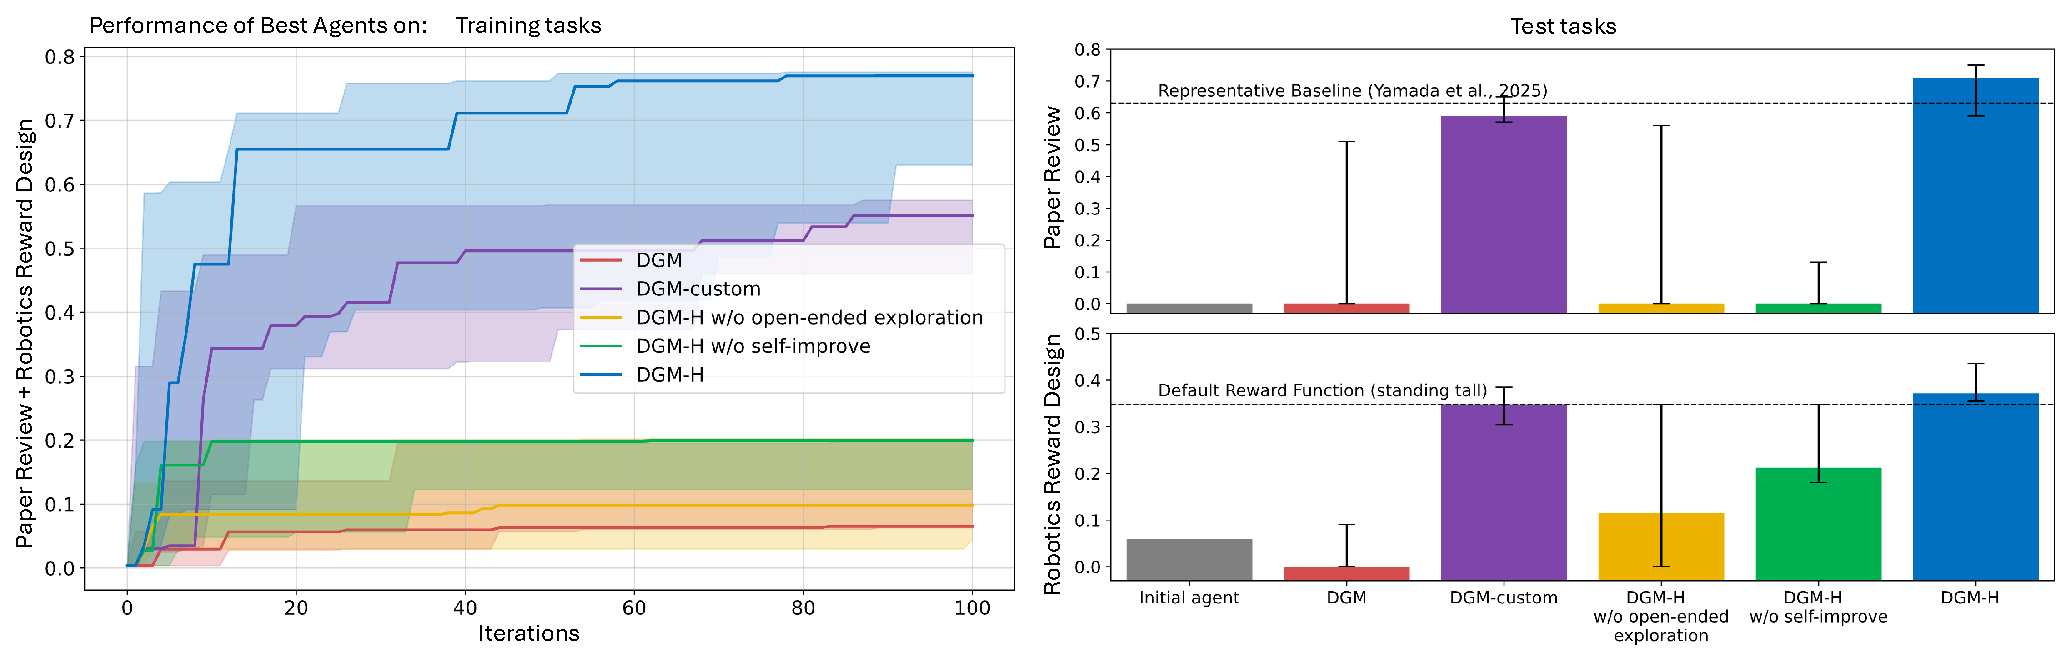
\includegraphics[width=\textwidth]{figures/ch_hyperagents/results_task.pdf}
\caption[Metacognitive self-modification and open-ended exploration enable the DGM-H to improve its performance]{\textbf{Metacognitive self-modification and open-ended exploration enable the DGM-H to continue making progress and improve its performance.} (Left) The DGM-H can optimize for diverse tasks within the same run and automatically discovers increasingly better task agents. (Right) The best discovered task agents, selected based on validation or training scores, are evaluated on test tasks in (Top-Right) paper review and (Bottom-Right) robotics reward design. The DGM-H outperforms baselines that lack metacognition (i.e., the original DGM), self-improvement, or open-ended exploration, showing that all components are essential for continual self-improvement.}
\label{fig:res-task}
\end{figure}

Beyond coding, we evaluate the DGM-H on paper review and robotics reward design jointly within a single run (Appendix~\ref{app:multi-domain}). All runs start from the same initial agent, which directly outputs the response from a single FM call (Appendix~\ref{app:initial-agent}), achieving a test-set score of 0.0 on paper review and 0.060 on robotics reward design (Figure~\ref{fig:res-task}). Starting from this initial agent, each method is run for 100 iterations.

\textbf{The original DGM requires domain-specific customization to generalize beyond coding.} Without customization, the original DGM achieves test-set performance of 0.0 on both domains, as expected given its coding-specific instruction-generation mechanism (Appendix~\ref{app:baseline-details}). When manually customized per domain, DGM-custom achieves 0.590 (CI: 0.570 -- 0.650) on paper review and 0.348 (CI: 0.305 -- 0.385) on robotics reward design, significantly outperforming the original DGM ($p < 0.05$) (Figure~\ref{fig:res-task}).

\textbf{Metacognitive self-modification enables sustained task improvement across domains.} The DGM-H substantially improves task performance over time in both domains, demonstrating effective improvement of the task agent. Importantly, these gains transfer to held-out test sets, indicating that improvements reflect general competence rather than overfitting to training tasks. On test tasks, DGM-H improves paper review performance from 0.0 (the initial agent) to 0.710 (CI: 0.590 -- 0.750) (Appendix~\ref{app:best-agents-paperreview}). Several top-performing agents outperform the open-sourced static baseline, which achieves 0.630 \citep{yamada2025ai}. On robotics reward design, DGM-H improves performance from 0.060 (the initial agent) to 0.372 (CI: 0.355 -- 0.436) (Appendix~\ref{app:best-agents-genesis}), surpassing the default reward function that directly optimizes the evaluation metric (0.348).

Qualitatively, the DGM-H moves beyond surface-level prompt tweaks toward structured decision machinery, such as multi-stage evaluation pipelines with checklists and decision rules for paper review, and an incrementally refined knowledge base of environment constraints and reward-scaling heuristics for robotics reward design (Appendix~\ref{app:qual-task}).

The DGM-H significantly outperforms the original DGM in both domains ($p < 0.05$), reflecting the limitations of the original DGM's fixed instruction-generation mechanism when applied to non-coding tasks (Figure~\ref{fig:res-task}). The DGM-H achieves higher median performance than DGM-custom on the test tasks in both domains, although the difference is not statistically significant ($p > 0.05$) (Figure~\ref{fig:res-task}). Notably, in the robotics reward design test task (i.e., design a reward function that trains the robot to maximize its torso height), the DGM-H almost always generates task agents that design reward functions inducing jumping behaviors, rather than getting stuck in the local optimum of standing tall. In contrast, DGM-custom often generates task agents that fail to escape this local optimum. This qualitative difference suggests that metacognitive self-modification can match or exceed handcrafted, domain-specific mechanisms.

\textbf{Both metacognitive self-modification and open-ended exploration are necessary for sustained improvement.}
DGM-H w/o self-improve \citep{huautomated} shows little to no improvement, achieving test-set performance of 0.0 (CI: 0.0 -- 0.130) on paper review and 0.213 (CI: 0.180 -- 0.348) on robotics reward design. The DGM-H significantly outperforms this baseline in both domains ($p < 0.05$) (Figure~\ref{fig:res-task}), demonstrating that the observed gains in the DGM-H are not solely due to task-level optimization under a fixed meta agent, but also arise from improvements in the self-modification process itself (i.e., the meta agent).
Similarly, DGM-H w/o open-ended exploration fails to achieve meaningful improvement, with test-set performance remaining at 0.0 (CI: 0.0 -- 0.560) on paper review and 0.116 (CI: 0.0 -- 0.348) on robotics reward design. The DGM-H significantly outperforms this baseline in both domains ($p < 0.05$) (Figure~\ref{fig:res-task}), highlighting the importance of open-ended, population-based search to create stepping stones for future improvements.

\subsection{Improving the Ability to Improve}
\label{sec:results-meta}

DGM-H's superior performance to DGM-H w/o self-improve shows that DGM-H improves the meta agent (i.e., its ability to self-modify and generate new agents) (Section~\ref{sec:results-task}). This section investigates whether these meta-level improvements are general rather than domain-specific. Specifically, we evaluate whether self-improvement strategies learned in one setting transfer to and accelerate learning in a different domain.

\textbf{Improvement@k metric.} To quantify a meta agent's ability to generate improved task agents, we introduce the improvement@k (imp@k) metric. Given an initial meta agent $M$, an initial task agent $A$, an agent-generation algorithm (e.g., DGM or DGM-H variants), and a fixed task, $M$ is allowed to generate up to $k$ new task agents from $A$ and its descendants using the specified algorithm. We define imp@k as the improvement in test performance from the initial task agent $A$ to the best-performing generated task agent (selected based on validation score) (Appendix~\ref{app:genk-metric}). Intuitively, imp@k measures how effectively a meta agent can produce improved variants within a limited number of iterations. To isolate the meta agent's ability to improve task agents from its ability to improve itself, we hold the meta agent fixed throughout the process (i.e., the agent responsible for generating new task agents is always the initial meta agent $M$), yielding DGM w/o self-improve and DGM-H w/o self-improve as the agent-generation algorithms. All experiments in this section run for 50 iterations, measuring imp@50.

\begin{figure}[ht]
\centering
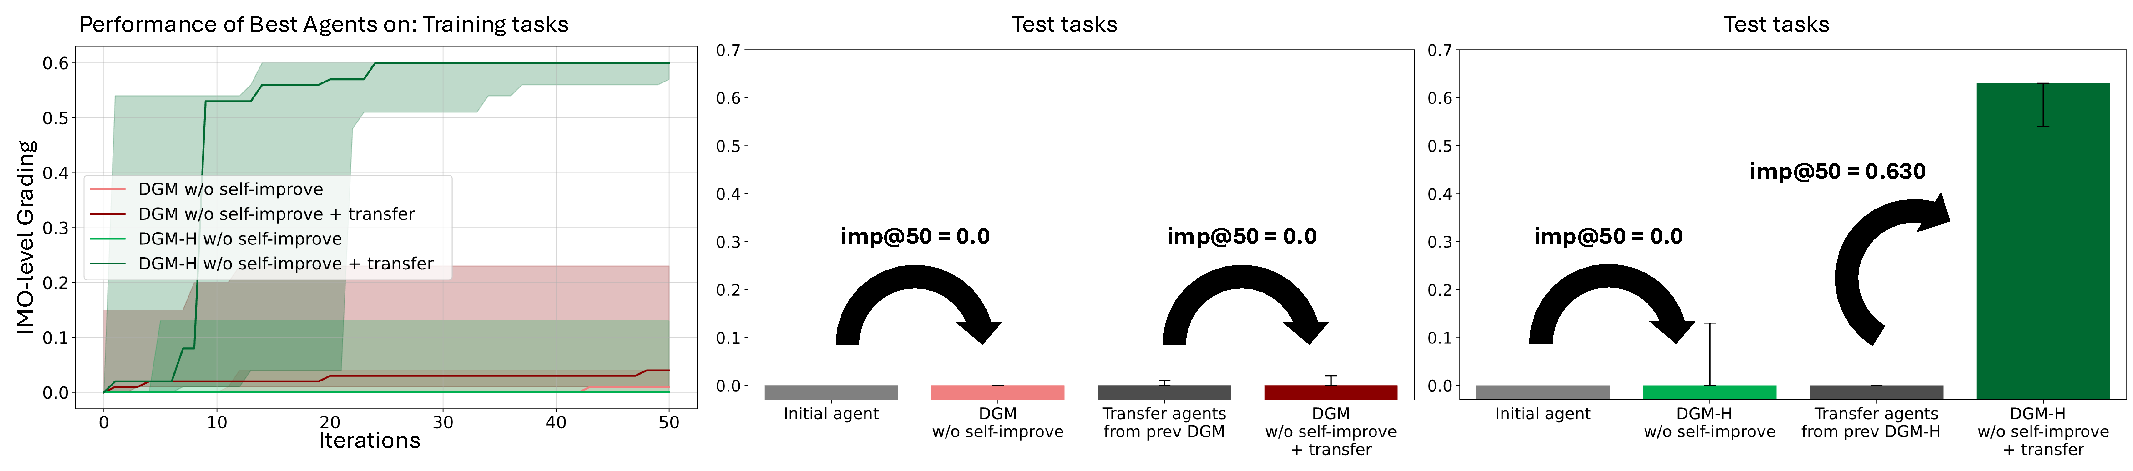
\includegraphics[width=\textwidth]{figures/ch_hyperagents/results_transfer.pdf}
\caption[Self-improvement strategies learned by the DGM-H transfer across domains]{\textbf{Self-improvement strategies learned by the DGM-H in one setting transfer to and accelerate learning in a different setting.} We measure an agent's ability to generate improved agents using imp@50, which takes as input a starting agent, an agent-generation algorithm, and an evaluation task. The algorithm is run for 50 iterations starting from the given agent, and imp@50 is defined as the performance gain of the best generated agent over the starting agent on the task. (Left, DGM w/o self-improve and DGM-H w/o self-improve) On Olympiad-level math grading, starting from the initial agent, both DGM w/o self-improve and DGM-H w/o self-improve achieve little to no improvement, showing that the initial agent has limited ability to generate better agents. (Left, DGM w/o self-improve + transfer) Starting from transfer agents, DGM w/o self-improve also achieves little improvement, showing that the original DGM does not learn transferable meta-level improvements. (Left, DGM-H w/o self-improve + transfer) In contrast, starting from transfer hyperagents, DGM-H w/o self-improve achieves substantial improvement, showing that hyperagents enable DGM-H to acquire transferable self-improvement strategies. (Middle) Regardless of starting from an initial agent or a transfer agent, DGM w/o self-improve yields imp@50 $\approx$ 0, showing that the original DGM does not improve the meta-level skill of generating improved agents. (Right) Starting from a transfer hyperagent, DGM-H w/o self-improve achieves large positive imp@50, showing that the self-improvement strategies learned by the DGM-H are general and transferable.}
\label{fig:res-transfer}
\end{figure}

\textbf{Neither the initial agent nor DGM-custom transfer agents can generate improved task agents in a new domain.}
We evaluate whether meta agents can generate improved task agents on a held-out domain, Olympiad-level math grading. Starting from the initial agent (Section~\ref{sec:exp-setup}), both DGM w/o self-improve and DGM-H w/o self-improve achieve imp@50 $\approx$ 0 (Figure~\ref{fig:res-transfer}), showing that the initial meta agent has little ability to generate improved task agents regardless of the agent-generation algorithm.
We next test whether self-improvements learned in prior DGM-custom runs on paper review and robotics reward design (Section~\ref{sec:results-task}) transfer to the new domain. From each run, we select a transfer agent based on the maximum performance gain achieved by its descendants, discounted by lineage depth to favor agents that reliably produce strong improvements within fewer steps (Appendix~\ref{app:transfer-selection}). For transfer, we carry over the entire agent implementation, using the transfer meta agent as the fixed agent responsible for generating new task agents and the transfer task agent as the starting point.
After 50 iterations, the DGM-custom transfer agents achieve imp@50 $\approx$ 0 (Figure~\ref{fig:res-transfer}). This shows that the gains observed with DGM-custom rely on domain-specific customizations rather than on general improvements in the ability to generate improved task agents.

\textbf{Hyperagents optimized in prior DGM-H runs demonstrate transferable ability to generate improved task agents in a new domain.}
We repeat the transfer experiments for the DGM-H to assess whether hyperagents enable the learning of general self-improvement mechanisms. From prior DGM-H runs on paper review and robotics reward design (Section~\ref{sec:results-task}), we select one transfer hyperagent per run using the same lineage-discounted criterion described above (Appendix~\ref{app:transfer-selection}). The transfer hyperagents (one from each of 5 repeated runs) achieve an initial test-set score of 0.0 (CI: 0.0 -- 0.0), reflecting the domain shift. After 50 iterations of DGM-H w/o self-improve starting from the transfer hyperagents, the best generated agents (selected based on validation score) achieve a test-set score of 0.630 (CI: 0.540 -- 0.630). This corresponds to a imp@50 of 0.630 (CI: 0.540 -- 0.630) (Figure~\ref{fig:res-transfer}). These results show that transfer hyperagents can generate improved agents in a previously unseen domain. When using DGM-H w/o self-improve as the agent-generation algorithm, imp@50 for the transfer agents is significantly higher than imp@50 for the initial agent ($p < 0.05$). This indicates that the transfer agents are substantially more effective at generating improved agents, and that the meta-improvements learned through DGM-H in one run are general and transferable, accelerating learning in a different domain.

We qualitatively attribute the observed transfer gains to a set of general-purpose meta-level capabilities that the DGM-H autonomously acquires during prior runs. In particular, the transfer hyperagents have features such as performance tracking and persistent memory, which allow them to reason about improvement as an ongoing process rather than as isolated code edits (Appendix~\ref{app:qual-meta}). As a result, even when transferred to an unseen domain, these hyperagents can quickly self-improve and make meaningful progress (Figure~\ref{fig:res-transfer}). This contrasts with DGM transfer agents, whose gains rely on domain-specific customizations and do not improve the underlying agent-generation process itself. These observations show that the DGM-H learns how to improve, yielding transferable self-improvement capability.

\subsection{Compounding Self-Improvements}
\label{sec:results-compound}

\begin{figure}[ht]
\centering
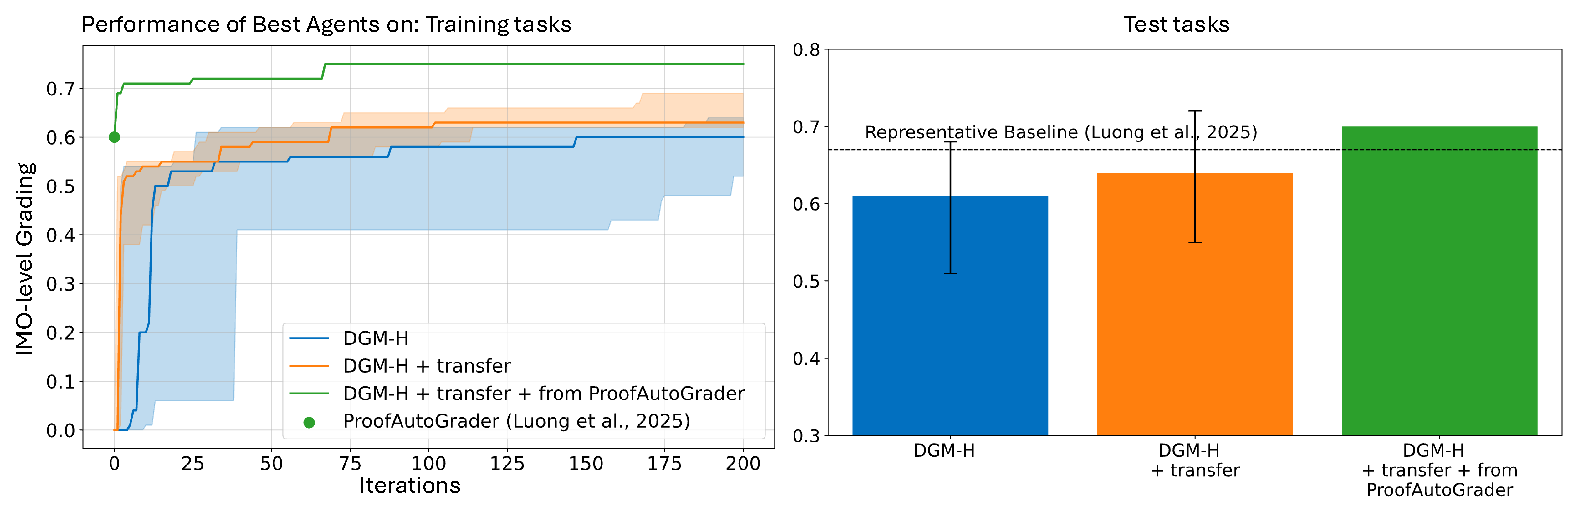
\includegraphics[width=0.9\textwidth]{figures/ch_hyperagents/results_transfercont.pdf}
\caption[Self-improvements learned by the DGM-H accumulate across domains and runs]{\textbf{Self-improvements learned by the DGM-H accumulate across domains and runs.} We continue running DGM-H on Olympiad-level math grading, starting from transfer hyperagents obtained in prior DGM-H runs, and compare this against DGM-H initialized from the initial agent and ProofAutoGrader. (Left) Initializing from transfer hyperagents leads to faster progress and higher final performance than initializing from the initial agent, indicating that previously learned self-improvements remain useful and continue to compound in a new domain. (Right) DGM-H initialized from a transfer agent and ProofAutoGrader achieves the highest test performance.}
\label{fig:res-transfer-cont}
\end{figure}

We investigate whether self-improvements learned by DGM-H in one setting continue to accumulate when DGM-H is run in a different setting. From prior DGM-H runs on the paper review and robotics reward design tasks (Section~\ref{sec:results-task}), we select transfer hyperagents using the same selection mechanism described earlier (Section~\ref{sec:results-meta}, Appendix~\ref{app:transfer-selection}). We then evaluate their ability to continue self-improving in a new domain, Olympiad-level math grading. After 200 iterations of DGM-H starting from these transfer agents (DGM-H + transfer), the best generated agents (selected based on validation score) achieve a test-set score of 0.640 (CI: 0.550 -- 0.720). Under the same experimental setup, DGM-H starting from the initial agent achieves a best test-set score of 0.610 (CI: 0.510 -- 0.680). Although the difference between DGM-H + transfer and DGM-H is not statistically significant ($p > 0.05$), DGM-H + transfer achieves a higher median performance and higher confidence intervals than DGM-H starting from the initial agent (Figure~\ref{fig:res-transfer-cont}). Notably, improvements at higher performance levels are increasingly difficult due to saturation effects (e.g., increasing performance from 0.7 to 0.8 is more challenging than from 0.0 to 0.1), making these gains meaningful despite their modest absolute magnitude. These results suggest that DGM-H's improvements are reusable and can potentially accumulate across runs, supporting the possibility of compounding self-improvement over time.

The representative static baseline for Olympiad-level math grading from IMO-GradingBench is ProofAutoGrader \citep{luong2025towards}. We initialize the DGM-H with ProofAutoGrader as the task agent and a transfer meta agent obtained from a prior DGM-H run (on paper review and robotics reward design), and then continue optimizing for Olympiad-level math grading. After 200 iterations, the best discovered agent achieves a test-set score of 0.700, outperforming ProofAutoGrader's score of 0.670 (Figure~\ref{fig:res-transfer-cont}). We then evaluate both the best discovered agent and ProofAutoGrader on the full IMO-GradingBench to obtain a more accurate estimate of the improvement. On the full IMO-GradingBench, the DGM-H improves ProofAutoGrader's accuracy from 0.561 to 0.601, and lowers the mean absolute error from 0.178 to 0.175 (Appendix~\ref{app:res-imograders}). We open-source this artifact to support future research and development (Appendix~\ref{app:best-agents-imograding}). These results show that the DGM-H can build on strong existing solutions and further improve their performance.

\section{Limitations and Conclusion}
\label{sec:conclusion}

Our results suggest that self-improvements can compound across different experimental settings, but this version of DGM-H has limitations that constrain truly unbounded progress.
First, it operates with a fixed task distribution. One direction is to co-evolve the task distribution by generating new tasks and curricula that adapt to the agent's capabilities \citep{clune2019ai, zhangomni, faldoromni, bolton2025sima}.
Second, components of the open-ended exploration loop (e.g., parent selection, evaluation protocols) remain fixed. Although hyperagents can modify their self-improvement mechanisms, they cannot alter the outer process that determines which agents are selected or how they are evaluated. Keeping these components fixed improves experimental stability and safety, but limits full self-modifiability. Enabling hyperagents to modify these outer-loop components and adapt their own search strategy and evaluation process is another promising direction for future work. Our preliminary results suggest such extensions are feasible (Appendix~\ref{app:res-parentselect}).

DGM-Hyperagents demonstrate that open-ended self-improvement can be made practical across diverse domains. Provided sufficient safety considerations are worked out, the DGM-H suggest a path toward self-accelerating systems that not only search for better solutions, but continually improve their ability to self-improve.

\section*{Acknowledgments}

We thank Andrew Budker and Ricardo Silveira Cabral for supporting this work, and Alisia Lupidi, Chenxi Whitehouse, John Quan, Lisa Alazraki, Lovish Madaan, Lucia Cipolina-Kun, Mattia Opper, Michael Dennis, Parth Pathak, Rishi Hazra, Roberta Raileanu, Sandra Lefdal, Shashwat Goel, Shengran Hu, Timon Willi, Tim Rockt\"{a}schel, and Yoram Bachrach for insightful discussions and feedback.

\textbf{Author Contributions.}
Jenny Zhang led the conceptualization of the study, conducted the experiments, and wrote the manuscript. Bingchen Zhao and Wannan Yang contributed to experimental design and execution. Jakob Foerster, Jeff Clune, Minqi Jiang, Sam Devlin, and Tatiana Shavrina provided feedback on the methodology and manuscript. All authors reviewed and approved the final manuscript.
